\documentclass[tikz,border=12pt]{standalone}
\usepackage{amsmath,amssymb}
\usetikzlibrary{arrows.meta,decorations.pathmorphing,calc}
\definecolor{ink}{HTML}{263145}
\definecolor{accent}{HTML}{4168B3}
\definecolor{warm}{HTML}{B77942}
\tikzset{every picture/.style={font=\small,text=ink},axis/.style={-{Stealth},thin,ink!65},curve/.style={accent,very thick},particle/.style={ink,thick,-{Stealth}}}
\begin{document}

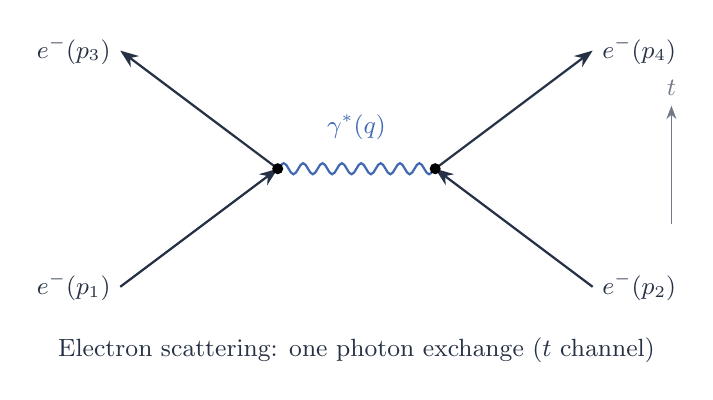
\begin{tikzpicture}
\coordinate (a) at (-1,0);\coordinate (b) at (1,0);
\draw[particle] (-3,-1.5)--(a);\draw[particle] (a)--(-3,1.5);
\draw[particle] (3,-1.5)--(b);\draw[particle] (b)--(3,1.5);
\draw[accent,thick,decorate,decoration={snake,amplitude=2pt,segment length=7pt}] (a)--(b);
\fill (a) circle (2pt);\fill (b) circle (2pt);
\node[left] at (-3,-1.5) {$e^-(p_1)$};\node[left] at (-3,1.5) {$e^-(p_3)$};
\node[right] at (3,-1.5) {$e^-(p_2)$};\node[right] at (3,1.5) {$e^-(p_4)$};
\node[accent,above=7pt] at (0,0) {$\gamma^*(q)$};
\draw[axis] (4,-.7)--(4,.8) node[above] {$t$};
\node at (0,-2.3) {Electron scattering: one photon exchange ($t$ channel)};
\end{tikzpicture}
\end{document}
